%----------------------------------------------------------------------------
\chapter*{Bevezető}
%----------------------------------------------------------------------------

A tőzsde egy központosított nyilvános szervezett piac, ahol különböző papírokkal, árukkal kereskedhetnek a brókerek. Régen a tőzsdéken nem használtak számítógépes rendszereket, a megbízások kötése minden esetben papíron, emberi erővel történt, így nyilván nem tudtak olyan sebességgel, akkora mennyiségben (annyi áruval) kereskedni mint manapság. Napjainkban a tőzsde elképzelhetetlen bonyolult számítógépes rendszerek nélkül, amik automatiksan végzik a megbízások kezelését és az ügyletek kötését, az áruk árát pedig valós időben követhetjük az bárhol a világon (emiatt ma már egyes számítások szerint a hálózati kábelek sebességén is múlhat egy-egy megbízás sikeressége).

\begin{figure}[!ht]
\centering
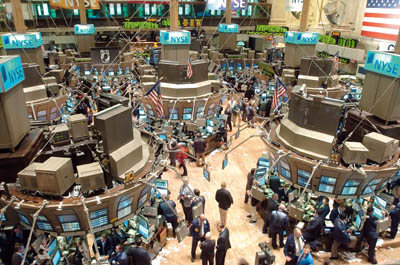
\includegraphics[width=70mm, keepaspectratio]{figures/tozsde.png}
\caption{Tőzsde}
\label{fig:kep_tozsde}
\end{figure}

A tőzsdéknek a következő tipusai léteznek:

\begin{itemize}
 \item árutőzsde
 \item értéktőzsde
 \subitem devizatőzsde
  \subitem értékpapírtőzsde
   \subitem hírpiac
\end{itemize}

Jelen web alapú tőzsdei applikációval egy értékpapír tőzsde működését kívántuk megvalósítani, úgy mint a megbízások, ügyletek kezelését, valós idejű értékpapír árfolyam kijelzés, számla adminisztráció.